% !TeX root = ../main.tex
% -*- coding: utf-8 -*-

\chapter{基于相关统计量的缺陷定位}
本章的研究内容主要针对一种重要的纠错性软件维护手段--缺陷定位。本章首先描述了缺陷定位对维护软件正确性
的作用,然后描述了基于程序谱的缺陷定位方法的一般过程。针对程序中可能存在多错误的问题,本文提出了基于
相关统计量的可疑度计算方法,在计算过程中尽可能避免多错误之间的相互影响。接着阐述了实验评估部分,描述
了实验设置,包括实验对象、对比实验和评价指标。在展示了实验结果和分析之后,对本章进行小结。

\section{引言}
软件系统在当今社会的军事、生活、教育等各个方面占据着重要的地位。随着人们对软件系统依赖性的不断增强,
软件系统失效往往给生活和经济带来巨大的损失,尤其在军事、航空等对可靠性有高要求的行业。软件缺陷是导致
软件失效的主要因素。软件缺陷的存在可能导致软件系统不能按照预期执行,从而造成误差甚至系统崩溃。为了保
证软件正确性,需要软件维护人员及时清除可能导致软件失效的缺陷。

当软件系统失效时,需要对软件系统进行纠错性软件维护,将潜在的软件缺陷清除。缺陷定位指的是当软件失效
时,查找并定位软件缺陷的过程,是纠错性软件维护的基础。虽然缺陷定位是纠错性软件维护的首要条件,但是人
工进行缺陷定位往往是一个冗长而繁复的过程。一方面人工缺陷定位通常依赖软件维护人员的经验和对软件系统的了解,
即使经验丰富的软件维护人员也很难迅速定位导致软件系统行为失效的根本原因。另一方面,针对大规模软件系统,人工缺陷定位所消耗的时间较长,软件维护人员需要充分理解源代码后逐步排查。

为了帮助软件维护人员查找缺陷,研究者们在自动缺陷定位的研究上投入了大量的工作。当前主要的缺陷定位方法
包括基于覆盖分析的方法、基于程序切片的方法、基于程序不变量的方法、基于模型检验的方法、基于状态变更的
方法等。其中大多数方法通过对软件系统的源代码或行为进行建模,查找与软件系统失效的代码。根据建模对象的
不同,传统的缺陷定位方法可以分为动态分析和静态分析两类。前者通过动态分析程序的行为,如执行路径或状态
等,查找相关代码;后者主要通过静态分析软件系统的源代码,从而分析与软件系统失效行为有关的程序元素。虽
然自动化缺陷定位的理论和技术得到了很大的发展,但当前的自动缺陷定位仍然面临两个挑战:

\begin{itemize}
      \item 随着需求的不断增加,软件系统越来越大,导致缺陷定位的效率降低。因此,适用于大规模软件系统的
   的缺陷定位越来越得到关注。
      \item 软件系统中潜在的缺陷可能不止一个,多个软件缺陷之间的相互影响可能导致自动缺陷定位的难度提
      高,准确度下降。尽管目前已经存在部分针对多缺陷的调试技术,但多缺陷的自动定位仍然是不小的挑战。
\end{itemize}

基于覆盖分析的缺陷定位方法,其核心思想是被失效用例执行越多、成功用例执行越少的代码可疑度越高。该类方
法通常只需要统计测试用例的执行结果和覆盖信息,并根据特定的公式计算代码的可疑度,不需要对软件系统的源
代码进行建模,因此计算复杂度低,在面对大规模软件系统时效率较高。然而,引起测试用例失效的软件缺陷可能
不止一个,忽略不同软件缺陷之间的相互影响,可能导致缺陷定位的准确性降低。其主要原因有两个方面:(1)
未被失效用例覆盖的代码可能也包含缺陷;(2)不同软件缺陷共同路径上的正确代码被失效用例覆盖的频率较
大,导致可疑度偏高。本文引入相关统计量的概念,通过将测试用例执行的覆盖信息作为特征,测试用例执行结果
作为标签,将原问题转化为数据挖掘问题,从而推测特征(代码)对执行结果的重要性。

本章具有以下贡献:
\begin{itemize}
      \item 本章提出了基于相关统计量的缺陷定位方法,从数据的角度分析测试用例的覆盖信息,利用特征选择
中特征对分类结果重要性的概念,将对测试用例执行结果影响较大的代码的可疑度提高。
      \item 该方法在传统的基于覆盖分析的缺陷定位方法上引入了相关统计量,同样不需要对源代码进行建模,计算复杂度较低。
      \item 针对多缺陷之间相互影响的问题,相关统计量为每个测试用例选择距离最近的同类和异类样本,计算
      测试用例在每个特征上距离同类和异类的距离,从而计算特征对测试执行结果的重要性。该方法在很大程度
      上避免了在衡量特征重要性时多错误之间的相互影响。
      \item 在开源软件系统上的实验证明,本章方法相比较传统启发式的基于覆盖分析的缺陷定位方法在准确性
      上具有一定的提升,通过提高缺陷查找效率缩短了纠错性维护的时间和人力成本。
\end{itemize}

\section{相关定义和问题描述}
基于覆盖分析的缺陷定位技术,通过程序谱的方式将测试用例的执行覆盖信息表现出来,并统计判断程序的执行结果,最后根据特定的可疑度计算公式逐个计算每个程序元素的可疑度,并按照可疑度由高至低排序推荐给软件维护人员。

\subsection{相关定义}
\begin{Definition}
      程序。程序$P$由代码序列表示,记作$P={e_1, e_2, e_3, ..., e_n}$,其中$e$表示程序元素,根据程序元素的不同,程序覆盖信息可分为关于语句、谓词、分支、变量定义-使用对等。
\end{Definition}

\begin{Definition}
      成功用例。当且仅当程序$P$的输出与预期预期输出一致时,称测试用例$t$为成功用例。
\end{Definition}

\begin{Definition}
      失效用例。当程序$P$的输出与预期预期输出不一致时,称测试用例$t$为失效用例。
\end{Definition}

\begin{Definition}
      程序谱。程序谱$S$由$m\times n$的矩阵构成,其中$m$为测试用例的个数,$n$为程序元素的个数。用$S_{ij}=1$表示第$i$个测试用例覆盖了第$j$个程序元素;$S_{ij}=0$表示第$i$个测试用例未覆盖第$j$个程序元素。
\end{Definition}

\begin{figure}[htp]
      \centering
      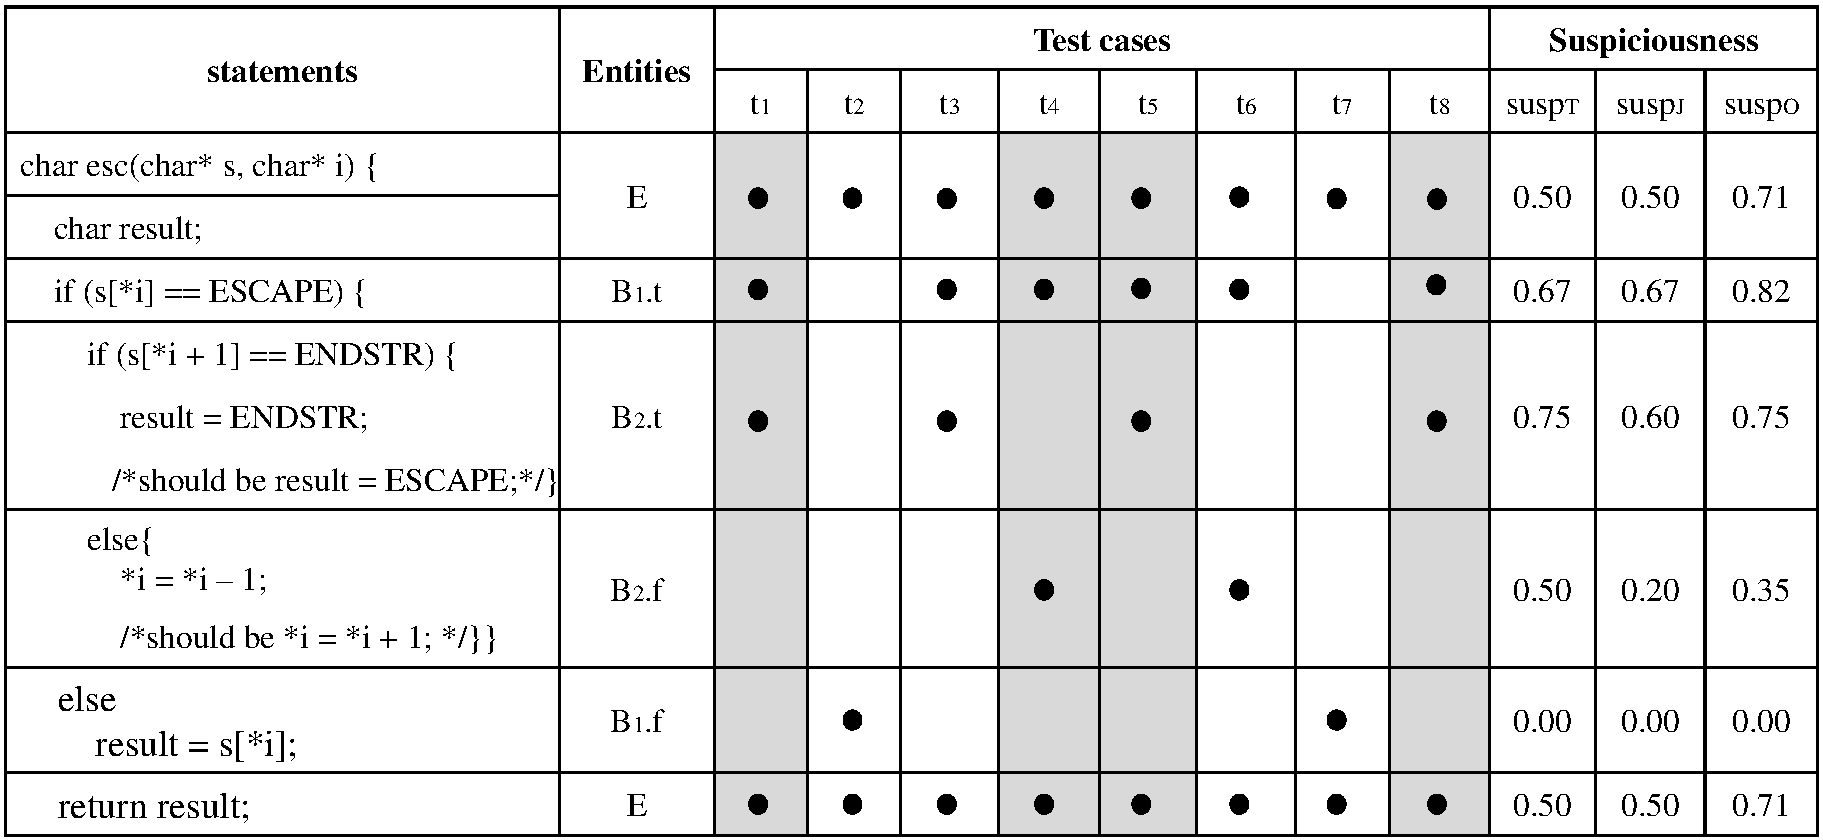
\includegraphics[width=0.95\linewidth]{spectra.pdf}
      \caption{示例程序的分支覆盖特征谱}
      \label{fig:spectra}
\end{figure}

本章以分支覆盖特征谱为例,提出了基于相关统计量的缺陷定位方法。值得注意的是,本章方法也同样适用于其它
程序元素。图~\ref{fig:spectra}是示例程序的分支覆盖特征谱,示例代码来自于西门子标准集
\footnote{http://sir.unl.edu/portal/index.php}。图~\ref{fig:spectra}中的示例代码共有2个嵌套的分支结
构,分别是$B_1$和$B_2$。对于每个分支结构,我们用分别用$t$和$f$来示意其两个分支,如$B_1.t$表示第一个
分支结构的真分支。根据分支情况将示例代码分为五个部分,可表示为$P = \{E, B_1.t, B_1.f, B_2.t,
B_2.f\}$,其中$E$表示程序的入口代码快。图~\ref{fig:spectra}中共有8个测试用例,每个测试用例的覆盖信息
表示为一列,黑色原型表示该测试用例覆盖了所对应的程序元素。灰色阴影的测试用例表示该用例的执行结果为失
效;反之则为成功用例。

图~\ref{fig:spectra}中使用三种经典的可疑度计算方法,分别是Tarantula~\cite{jones2005empirical}、
Jaccard~\cite{abreu2007accuracy}和Ochiai~\cite{abreu2007accuracy},可疑度计算公式如下:
\begin{eqnarray}
 susp_T = \frac{\frac{a_{11}}{a_{11}+a_{01}}}{\frac{a_{11}}{a_{11}+a_{01}}+\frac{a_{10}}{a_{10}+a_{00}}}, \label{eq:tar}\\
susp_J = \frac{a_{11}}{a_{11}+a_{01}+a_{10}}, \label{eq:jac}\\
susp_O = \frac{a_{11}}{\sqrt{(a_{11}+a_{01})\times(a_{11}+a_{10})}}, \label{eq:och}
\end{eqnarray}

上述公式中的四个变量均用来描述程序元素覆盖与否信息与执行结果之间的关系:
\begin{itemize}
  \item $a_{00}$表示测试用例被成功执行但未覆盖某个程序元素;
  \item $a_{01}$表示测试用例执行失效且未覆盖某个程序元素;
  \item $a_{10}$表示测试用例被成功执行且覆盖某个程序元素;
  \item $a_{11}$表示测试用例执行失效且覆盖了某个程序元素。
\end{itemize}

\subsection{问题描述}
传统的基于覆盖分析的缺陷定位方法,基于启发式的思想使用特定公式计算程序元素的可疑度,其优点在于计算复杂度低,面对大规模软件系统的效率较高,但也存在一定的问题:由于基于覆盖分析的方法不对程序源代码进行建模,而是从统计的角度根据代码被失效和成功覆盖的频率推测代码的可疑度,因此对于存在多错误的失效用例,难以区分导致用例失效的不同缺陷。一方面,成功执行的用例可能覆盖缺陷但却未触发缺陷;另一方面,失效执行的用例可能未覆盖缺陷代码,图~\ref{fig:spectra}中



\section{基于相关统计量的缺陷定位算法}
\subsection{特征表示}
\subsection{相关统计量}
具体来说,Relief为每个测试用例寻找距离最近的同类和异类样本,距离同类越近、距离异类越远的特征被认为越能够区分不同类别的样本。
\subsection{可疑度计算方法}
\section{实验设置}
\subsection{实验对象}
\subsection{对比实验}
\subsection{评价指标}
\section{实验结果与分析}
\subsection{实验结果}
\subsection{分析与讨论}
\section{本章小结}
